%//==============================--@--==============================//%
\subsection[3.1 Equações básicas de Controlo ]{\hspace*{0.075 em}\raisebox{0.2 em}{$\pmb{\drsh}$} Equações básicas de Controlo}
\label{sec:eq-base-control}
\noindent Considerando o seguinte diagrama de blocos reunem-se de seguida um conjunta de equações com respeito aos sistemas de malha aberta e malha fechada:

\begin{figure}[H]
    \centering
    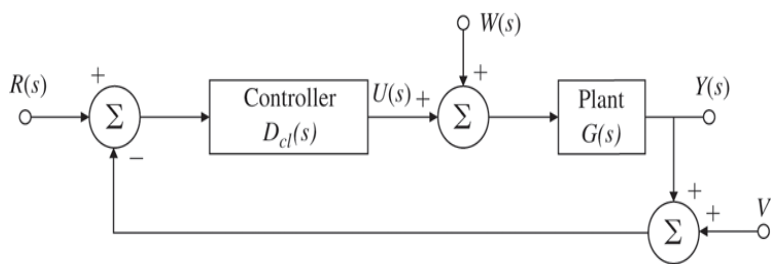
\includegraphics[width = 0.8\linewidth]{img/3/feedback-loop.png}
    \caption{diagrama de blocos generalista de um dado sistema}
    \label{fig:feed-loop}
\end{figure}

\noindent Supondo o sistema em \textbf{malha aberta}, podemos garantir a a equação de saída do sistema com recurso ao princípio da sobreposição. Neste sentido o sistema é linear com a seguinte saída:
$$
    Y_{ol} = G D_{ol} R - G W
$$
\noindent Onde $W$ são as perturbações induzidas pelo meio.

\vspace{1 em}
\noindent Consequentemente, a equação do erro, diferença entre a entrada de referência e a saída, é dada por:
$$
\begin{aligned}
    E_{ol} &= R - Y_{ol}\\
    &= R - G D_{ol} R - G W\\
    &= R[1 - G D_{ol}] - G W
\end{aligned}
$$

\noindent  função de transferência em cadeia aberta é portanto:
$$
    \boxed{T(s) = G(s) D_{ol}(s)}
$$

\noindent Supondo agora o sistema em \textbf{malha fechada}. Existem três entradas externas: a referência, $R$, que se espera que a saída siga; a perturbação do meio, $W$, que se espera que o controlo contrarie para não perturbar a saída; e o ruído do sensor, $V$, que se espera que o controlador ignore:
$$
\begin{aligned}
    Y_{cl} = \dfrac{GD_{cl}}{1 + GD_{cl}}R + \dfrac{G}{1 + GD_{cl}}W + \dfrac{GD_{cl}}{1 + GD_{cl}}V\\
    U_{cl} = \dfrac{D_{cl}}{1 + GD_{cl}}R + \dfrac{GD_{cl}}{1 + GD_{cl}}W + \dfrac{D_{cl}}{1 + GD_{cl}}V
\end{aligned}
$$

\noindent Onde o erro é novamente dado por $E_{cl} = R - Y_{cl}$ e a função de transferência é
$$
    \boxed{T(s) = \dfrac{D_{cl}}{1 + GD_{cl}}}
$$

%//==============================--@--==============================//%
\newpage
\subsection[3.2 Objectivos Gerais de um Sistema de Controlo]{\hspace*{0.075 em}\raisebox{0.2 em}{$\pmb{\drsh}$} Objectivos Gerais de um Sistema de Controlo}
\label{sec:obj-gerais-cont}

\begin{itemize}
\item Bom seguimento do sinal de referência --- a variável que se pretende controlar deve tomar valores tão próximos quanto possível dos valores desejados expressos pela referência, ou seja, o erro deve ser pequeno
\item Boa rejeição dos efeitos das perturbações, incluindo ruído
\item Rapidez da resposta, quer no seguimento, quer na rejeição de perturbações
\item Estabilidade
\item Pequena sensibilidade à variação de parâmetros
\item Robustez de estabilidade
\begin{itemize}
    \item Relativamente à variação de parâmetros
    \item Relativamente a incertezas no modelo do sistema físico no qual se baseou o projeto de controlador
\end{itemize}
\item Dinâmica não modelada, resultante, por exemplo, da aproximação de um sistema de 3ª ordem por um modelo mais simples de 2ª ordem
\end{itemize}

%//==============================--@--==============================//%
\subsubsection[3.2.1 Seguimento do sinal de referência]{$\pmb{\rightarrow}$ Seguimento do sinal de referência}
\noindent Se considerarmos apenas o seguimento da entrada de referência e definirmos $W = V = 0$ então a equação para o erro é simplesmente:

$$
    \dfrac{E}{R} = \dfrac{1}{1 + GD_{cl}}
$$
\noindent Considerando entradas polinomiais, admitimos que $R = \frac{1}{s^{k + 1}}$. Tomando um sistema mecânico como base para uma nomenclatura genérica de referência, chamamos às entradas em degrau para as quais $k = 0$, "posição", às entradas em rampa para as quais $k = 1$, "velocidade" e  às entradas para as quais $k = 2$, "aceleração. A aplicação do Teorema do Valor Final à fórmula de erro indica o seguinte resultado:

$$
    \begin{aligned}
        e_{ss} &= \lim_{s \to 0} s E(s)\\
        &= \lim_{s \to 0} \dfrac{s}{1 + GD_{cl}} \cdot \dfrac{1}{s^{k + 1}}
    \end{aligned}
$$

\noindent Consideramos primeiro um sistema para o qual não há pólo na origem, e uma entrada em degrau unitário para a qual $R(s) = \frac{1}{s}$. o limite acima descrito é reduzido para:
$$
    \lim_{s \to 0} \dfrac{s}{1 + GD_{cl}} \cdot \dfrac{1}{s} = \dfrac{1}{1 + GD_{cl}(0)} = \dfrac{1}{1 + K_p}
$$

\noindent Repare-se que a equação acima produz o erro estático de posição e que, se a entrada fosse um polinómio de grau superior a 1, o erro resultante cresceria sem limites. Um polinómio de grau 0 é o grau mais elevado que um sistema de tipo 0 pode seguir.

\vspace{1 em}
\noindent Supondo agora uma visão mais generalista, iremos escrever a função de transferência em malha aberta da seguinte forma:

$$
    GD_{cl} = \dfrac{GD_{clo}}{s^n}
$$
\noindent Se o sistema não possuir um pólo na origem então $n = 0$, se possuir um, $n = 1$, $\dots$

\noindent Assim, reescrevendo a equação do erro:
$$
    \begin{aligned}
        e_{ss} &= \lim_{s \to 0} s E(s)\\
        &= \lim_{s \to 0} \dfrac{s}{1 + \dfrac{GD_{clo}}{s^n}} \cdot \dfrac{1}{s^{k + 1}}\\
        &= \lim_{s \to 0} \dfrac{s^n}{s^n + K_N}\dfrac{1}{s^k}
    \end{aligned}
$$

\noindent Da equação acima, é fácil observar que se $n > k$ então $e_{ss} = 0$ e que se $n < k$ então $e_{ss} \to \infty$ e se $k = n \neq 0$, então $e_{ss} = 1/K_n$. Assim:

\begin{itemize}
    \item Se $n = k = 0$, $K_0 = K_p$ é denominada de "constante de posição", e o sistema é classificado como de tipo 0.
    \item Se $n = k = 0$, $K_1 = K_v$ é denominada de "constante de velocidade", e o sistema é classificado como de tipo 1.
    \item Se $n = k = 2$, $K_2 = K_a$ é denominada de "constante de aceleração", e o sistema é classificado como de tipo 2.
\end{itemize}

\begin{table}[h!]
\centering
\renewcommand{\arraystretch}{2.7} % Increase vertical cell padding
\begin{tabular}{|c|c|c|c|}
\hline
 & $n = 0$ & $n = 1$ & $n = 2$ \\
\hline
$k = 0$ & $\dfrac{1}{1 + K_p}$ & $0$ & $0$ \\
\hline
$k = 1$ & $+\infty$ & $\dfrac{1}{K_v}$ & $0$ \\
\hline
$k = 2$ & $+\infty$ & $+\infty$ & $\dfrac{1}{K_a}$ \\
\hline
\end{tabular}
\label{tab:system_types}
\end{table}

\noindent De forma sucinta, os coeficientes de erro estático podem ser determinados da seguinte forma:

$$
    \begin{aligned}
        K_p &= \lim_{s \to 0}G D_{cl}(s),\;\, n = 0\\[4pt]
        K_v &= \lim_{s \to 0}s G D_{cl}(s),\;\, n = 1\\[4pt]
        K_a &= \lim_{s \to 0}s^2 G D_{cl}(s),\;\, n = 2
    \end{aligned}
$$

%//==============================--@--==============================//%
\newpage
\subsubsection[3.2.2 Rejeição de perturbações]{$\pmb{\rightarrow}$ Rejeição de perturbações}
\noindent Supondo agora o seguinte diagrama de blocos simplificado:

\begin{figure}[H]
    \centering
    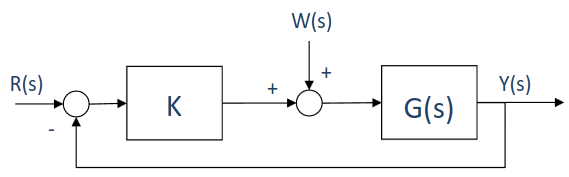
\includegraphics[width = 0.9\linewidth]{img/3/feedback-loop-simp.png}
    \caption{diagrama de blocos simplificado}
    \label{fig:feed-loop-simp}
\end{figure}

\noindent É de fácil observação que a atenuação do efeito de $W$ é mais versátil supondo o modelo em malha fechada:

$$
    Y(s) = \dfrac{KG(S)}{1 + KG(s)}R(s) + \boxed{\dfrac{G(s)}{1 + KG(s)}W(s)}
$$

\noindent A influência de $W(s)$ é atenuada através do incremento de $K$. \textbf{A saída é tanto menos afetada por $W$ quanto maior for o ganho do controlador, $K$}. Assim, é possível enunciar as seguintes observações:

\begin{itemize}
    \item Boa rejeição da perturbação $W$ aumentar $|KG(jw)|$
    \item Bom seguimento da referência r (erro pequeno) aumentar $|KG(jw)|$
\end{itemize}

\noindent Supondo agora um modelo que inclua a adição de uma componente $V$ de ruído (de forma análoga à verificada na \hyperref[fig:feed-loop]{fig. 6}), obtemos a seguinte expressão de saída:

$$
    Y(s) = \dfrac{KG(S)}{1 + KG(s)}R(s) + \boxed{\dfrac{G(s)}{1 + KG(s)}W(s) + \dfrac{KG(S)}{1 + KG(s)}V(s)}
$$

\noindent O ruído, cuja \textbf{mitigação passa pela diminuição de $K$}, apresenta habitualmente componentes espectrais de mais alta frequência do que as do sinal de referência. Assim, tipicamente é realizada a seguinte estratégia de controlo:

\begin{itemize}
    \item A baixas frequências, $|KG(jw)| >> 1$
    \item A altas Frequências (nas quais encontramos a banda do ruído) $|KG(jw)| <<1$
    \item Nas frequências intermédias as condições a impor ao ganho estão relacionadas com a
estabilidade em cadeia fechada (já que a alteração do ganho provoca alterações na localização dos pólos do sistema). 
\end{itemize}

%//==============================--@--==============================//%